\problemname{Mancala}

\emph{Mancala} is a family of board games played around the world, sometimes
called \emph{sowing} games, or \emph{count-and-capture} games, which describes the
game play.  One simple variant is a solitaire game called \emph{Tchoukaillon}
which was described by V\'eronique Gautheron.  \emph{Tchoukaillon} is played on
a board with an arbitrary number of bins numbered $1, 2, \ldots,$  containing
$b[1], b[2], ... ,$ counters respectively and an extra empty bin called
the Roumba on the left.

% insert image 1
\begin{figure}[!h]
    \begin{center}
        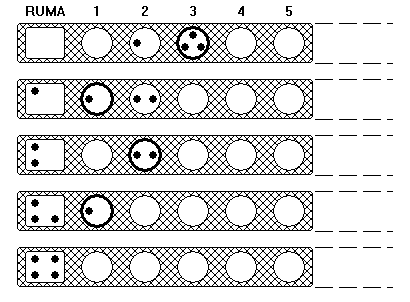
\includegraphics[]{e1.png} \\
    \end{center}
\end{figure}

A single play consists on choosing a bin, $n$, for which $b[n] = n$ (indicated
by the darker circles in the diagram) and distributing the counters one
per bin to the bins to the left including the \emph{Roumba} (getting the next
diagram below in the figure above).  If there is no bin where $b[n] = n$,
then the board is a losing board.

If there is a sequence of plays which takes the initial board distribution
to one in which every counter is in the \emph{Roumba}, the initial distribution
is called a winnable board.  In the example above, $0,1,3,\ldots$ is a
winnable board (the ``$\ldots$'' indicates all the bins to the right of
bin 3 contain 0).  For each total number of counters, there is a unique
distribution of the counters to bins to make a winnable board for that
total count (so $0,1,3,\ldots$ is the only winnable board with $4$ counters).

Write a program which finds the winnable board for a total count input.

\section*{Input}

The first line of input contains a single integer $P$, ($1 \le P \le 1000$),
which is the number of data sets that follow.  Each data set should be
processed identically and independently.

Each data set consists of a single line of input.  It contains the data
set number, $K$, followed by a single space, followed by the total count $N$
($1 \le N \le 2000$) of the winnable board to be found.

\section*{Output}

For each data set there will be multiple lines of output.  The first
line of output contains the data set number, $K$, followed by a single
space, followed by the index of the last bin, $B$, with a non-zero count.
Input will be chosen so that $B$ will be no more than $80$.  The first line
of output for each dataset is followed by the bin counts $b[1], b[2], … , b[B]$,
10 per line separated by single spaces.

